\chapter{Counters, Clock Dividers and State Machines}
\label{ch:fsm}

With flip-flops and timing understood, we can build circuits that step through sequences: counters, circuits that make slower clocks from faster ones, and finite state machines, which are the ``brains'' of almost every control circuit. Candidates report questions on all three: clock dividers with particular duty cycles, counting flip-flops in a counter, the minimum flip-flops for a traffic-light controller, and sequence detectors.

\section{Counters}

A \term{counter} is a register that adds 1 on every clock edge. An $n$-bit counter steps through $0, 1, 2, \ldots, 2^n - 1$ and then wraps back to 0.

\paragraph{Synchronous counter.} A register plus an adder: $Q^+ = Q + 1$. All flip-flops share one clock and change together. This is the standard design.

\paragraph{Ripple counter.} A chain of toggle flip-flops in which each flip-flop's output clocks the next. The first flip-flop toggles on every clock edge, so its output is a square wave at half the clock frequency. The second toggles on every edge of the first, so it runs at a quarter of the clock frequency, and so on. Ripple counters are small, but each stage adds a clock-to-Q delay, so the bits do not change at the same instant. Reading the count while it ripples gives wrong values briefly.

\begin{bigidea}
Each bit of a binary counter runs at half the frequency of the bit below it. Bit $k$ (counting from bit 0) is a square wave at $f_{clk}/2^{k+1}$. The most significant bit of an $n$-bit counter has frequency $f_{clk}/2^n$ and period $2^n \cdot T_{clk}$.
\end{bigidea}

\begin{worked}{how many flip-flops in the counter?}
An engineer measures a binary counter: the clock period is 2\,ns, and the counter's most significant output has a period of 128\,ns. How many flip-flops does the counter have?

The MSB period is $2^n$ times the clock period: $2^n = 128/2 = 64$, so $n = 6$ flip-flops.
\end{worked}

\begin{onoa}
A reported question gives two measured times, $A = 2$\,ns and $B = 128$\,ns, and asks for the number of flip-flops in a binary counter. With $A$ as the clock period and $B$ as the period of the top bit, the answer is $\log_2(128/2) = 6$. Use the same reasoning for any variant: the frequency ratio between the clock and the top bit is $2^n$.
\end{onoa}

\paragraph{Mod-$N$ counters.} A counter that counts $0$ to $N-1$ and then wraps to 0 is a \term{mod-$N$ counter}. It needs $\lceil \log_2 N \rceil$ flip-flops: a decimal digit counter (mod 10) needs 4. It is built as a normal counter with a comparator that resets it to 0 when it reaches $N - 1$.

\paragraph{Counters with enable.} Often a counter should only count when an enable input is 1: $Q^+ = EN\;?\;Q+1 : Q$.

\begin{worked}{a counter with an enable input}
A counter starts at 0 and increments on each rising clock edge \emph{only if} input $X = 1$ at that edge. The clock is 8\,kHz; $X$ is a 2\,kHz square wave. Assume $X$ is 1 at clock edges 1 and 2, 0 at edges 3 and 4, 1 at edges 5 and 6, and so on.

The clock is 4 times faster than $X$, so each period of $X$ spans 4 clock edges: 2 with $X = 1$ and 2 with $X = 0$. After edge 7, the counter has incremented at edges 1, 2, 5 and 6: the count is 4. After edge 10, add edges 9 and 10: the count is 6.
\end{worked}

The answer depends on how the two waveforms line up, so read the question's timing diagram carefully: which edges see $X = 1$ is the whole problem.

\section{Clock dividers}

A \term{clock divider} makes a slower clock from a faster one. It is one of the most commonly reported interview topics.

\subsection*{Divide by 2}

Connect a D flip-flop's $\nt{Q}$ to its own $D$ (or use a T flip-flop with $T = 1$). Each rising edge flips the output, so the output completes one full cycle every two clock cycles: half the frequency, with a perfect 50\% duty cycle.

\begin{worked}{a toggle flip-flop}
A 25\,kHz clock drives a T flip-flop with $T = 1$ and its asynchronous set and clear inputs tied inactive. The output is a 12.5\,kHz square wave. A second such stage, clocked by the first, gives 6.25\,kHz.
\end{worked}

A chain of $n$ such stages divides by $2^n$.

\subsection*{Divide by an even number}

To divide by $N = 2M$ with a 50\% duty cycle, count clock edges from 0 to $M - 1$ and toggle the output each time the count wraps. For divide-by-6, toggle every 3 cycles: the output is high for 3 cycles and low for 3.

\subsection*{Divide by an odd number with a 50\% duty cycle}

Odd division is harder, because $N$ cycles cannot be split into two equal whole numbers of cycles. The trick is to use \emph{both} clock edges. For divide-by-3:

\begin{enumerate}
  \item Build a mod-3 counter on the rising edge (states 0, 1, 2).
  \item Make a signal $P$ that is 1 during state 0: high for 1 cycle out of 3 (a 33\% duty cycle).
  \item Make $N$, a copy of $P$ delayed by half a cycle, by sampling $P$ with a flip-flop on the \emph{falling} clock edge.
  \item Output $P$ OR $N$. It is high for $1 + \tfrac12 = 1.5$ cycles out of 3: exactly 50\%.
\end{enumerate}

\begin{figure}[h]
\centering
\begin{tikztimingtable}[timing/slope=0.05, xscale=1.8, yscale=1.2]
$CLK$   & H L H L H L H L H L H L \\
count   & 2D{0} 2D{1} 2D{2} 2D{0} 2D{1} 2D{2} \\
$P$     & 2H 4L 2H 4L \\
$N$     & 1L 2H 4L 2H 3L \\
$P + N$ & 3H 3L 3H 3L \\
\extracode
\begin{pgfonlayer}{background}
\vertlines[help lines]{0,2,4,6,8,10}
\end{pgfonlayer}
\end{tikztimingtable}
\caption{Divide-by-3 with a 50\% duty cycle. $P$ comes from rising edges (gridlines); $N$ is $P$ delayed to the next falling edge; their OR is high for 1.5 of every 3 clock cycles.}
\label{fig:div3}
\end{figure}

The same method divides by any odd $N$: make $P$ high for $(N-1)/2$ cycles out of $N$, delay it half a cycle, and OR. For divide-by-5, $P$ is high for 2 cycles; the OR is high for 2.5 cycles out of 5.

\subsection*{Divide by 2 with a 25\% duty cycle}

Take the divide-by-2 output $Q$ (high for one full clock period, low for the next) and combine it with the clock itself. Inside each period in which $Q$ is high, the clock is high for half and low for half. ANDing $Q$ with the clock, or with the inverted clock, keeps only one half: a pulse one half-period wide every two periods, which is a 25\% duty cycle at half the frequency.

Which version? $Q$ changes just \emph{after} each rising clock edge (by $t_{cq}$). With $Q \cdot CLK$, at the rising edge where $Q$ falls, the clock rises a moment before $Q$ drops, producing a brief glitch. With $Q \cdot \nt{CLK}$, the inverted clock falls at that edge before $Q$ changes, so no glitch can occur. The glitch-free answer is
\[
  \text{OUT} = Q \cdot \nt{CLK}.
\]

\begin{onoa}
Reported clock-divider questions include divide-by-2 with a 25\% duty cycle and divide-by-3 with a 50\% duty cycle (``bonus for 50\% duty cycle''), followed by many follow-up questions about the design. Be ready to draw the waveforms, explain why odd division needs the falling edge, and point out glitch risks when gating a clock with logic.
\end{onoa}

\paragraph{A caution about logic on clocks.} Combining clocks with ordinary gates can create glitches, and a glitch on a clock is catastrophic: flip-flops see it as an extra edge. Real designs use special glitch-free clock-gating cells and clock muxes, and keep clock logic to a minimum.

\section{Finite state machines}

A \term{finite state machine} (FSM) is a circuit that remembers which of a fixed set of \term{states} it is in, and moves between states according to its inputs. Traffic lights, vending machines, communication protocols, and the control unit of every processor are FSMs.

Every synchronous FSM has the same three parts (Figure~\ref{fig:fsmblock}):
\begin{itemize}
  \item a \term{state register}: flip-flops holding the current state;
  \item \term{next-state logic}: combinational logic computing the next state from the current state and inputs;
  \item \term{output logic}: combinational logic computing the outputs.
\end{itemize}

\begin{figure}[h]
\centering
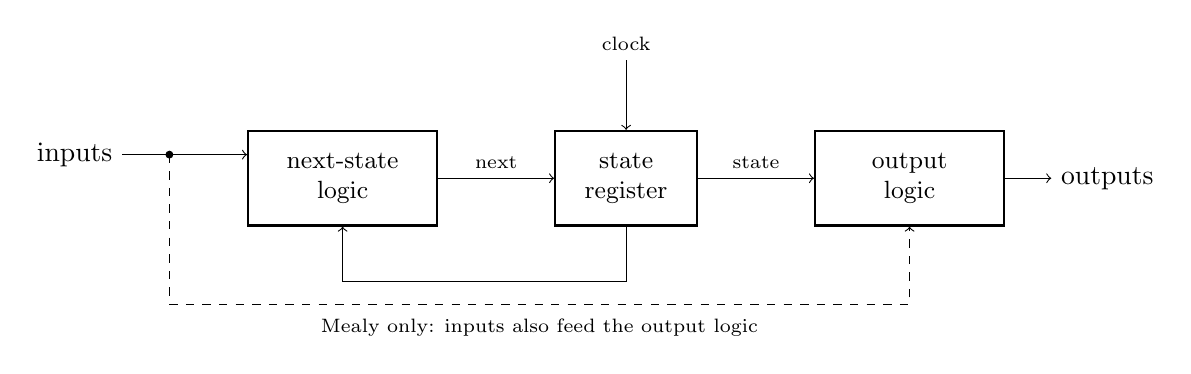
\begin{tikzpicture}[box/.style={draw,thick,minimum height=1.2cm,align=center,font=\small}]
  \node[box,minimum width=2.4cm] (ns) at (0,0) {next-state\\logic};
  \node[box,minimum width=1.8cm] (sr) at (3.6,0) {state\\register};
  \node[box,minimum width=2.4cm] (ol) at (7.2,0) {output\\logic};
  \draw[->] (-2.8,0.3) node[left]{inputs} -- ([yshift=0.3cm]ns.west);
  \draw[->] (ns) -- node[above,font=\scriptsize]{next} (sr);
  \draw[->] (sr) -- node[above,font=\scriptsize]{state} (ol);
  \draw[->] (ol) -- ++(1.8,0) node[right]{outputs};
  \draw[->] (sr.south) -- ++(0,-0.7) -| (ns.south);
  \draw[->] (3.6,1.5) node[above,font=\scriptsize]{clock} -- (sr.north);
  \fill (-2.2,0.3) circle (0.05);
  \draw[->,dashed] (-2.2,0.3) -- (-2.2,-1.6) -- (7.2,-1.6) -- (ol.south);
  \node[font=\scriptsize] at (2.5,-1.9) {Mealy only: inputs also feed the output logic};
\end{tikzpicture}
\caption{Structure of a finite state machine.}
\label{fig:fsmblock}
\end{figure}

\paragraph{Moore versus Mealy.}
\begin{itemize}
  \item In a \term{Moore machine}, the outputs depend only on the current state. Outputs are stable for a whole cycle and glitch-free, but they react to an input one cycle later.
  \item In a \term{Mealy machine}, the outputs depend on the current state \emph{and} the current inputs. Mealy machines react within the same cycle and often need fewer states, but their outputs can glitch when the inputs do.
\end{itemize}

\paragraph{State encoding.} The states must be given binary codes:
\begin{itemize}
  \item \textbf{Binary}: number the states $0, 1, 2, \ldots$. Fewest flip-flops: $\lceil\log_2(\text{number of states})\rceil$.
  \item \textbf{One-hot}: one flip-flop per state, exactly one of them 1. More flip-flops, but the next-state logic is simple and fast. Popular in FPGAs.
  \item \textbf{Gray}: consecutive states differ by one bit, which reduces switching power and glitches.
\end{itemize}

\section{Example: how many flip-flops for a traffic light?}

\begin{worked}{the minimum flip-flops for a traffic-light FSM}
A traffic light stays green for 30\,s, yellow for 5\,s and red for 25\,s, then repeats. The controller's clock has a 1\,s period, and the FSM must count the seconds itself (no separate timer). What is the minimum number of flip-flops?

Every second of the 60-second cycle must be a distinct state, because the machine must know how long it has been in each color. That is $30 + 5 + 25 = 60$ states. Minimum flip-flops: $\lceil \log_2 60 \rceil = 6$ (since $2^5 = 32 < 60 \le 64 = 2^6$).
\end{worked}

A common alternative design uses a 3-state color FSM (2 flip-flops) plus a separate countdown timer big enough for 30 (5 flip-flops): 7 flip-flops in total. It is often cleaner, but it is not the minimum. Read whether the question asks for the minimum.

\begin{onoa}
A reported question asks for the minimum number of flip-flops for a traffic-light FSM, given the green, yellow and red durations and a clock period. The method: total cycles in one full loop $=$ (sum of the durations) / (clock period); minimum flip-flops $= \lceil \log_2(\text{total cycles}) \rceil$.
\end{onoa}

\section{Example: a sequence detector}

A \term{sequence detector} watches a serial input, one bit per clock cycle, and outputs 1 when a particular pattern has just arrived. With \term{overlap}, the end of one match may also be the start of the next.

\begin{worked}{detecting 1011 with overlap (Mealy)}
Each state records how much of the pattern 1011 has been seen so far:
\begin{itemize}
  \item S0: nothing useful yet.
  \item S1: seen ``1''.
  \item S2: seen ``10''.
  \item S3: seen ``101''.
\end{itemize}
The transitions, written as input/output:
\begin{center}
\begin{tabular}{lll}
\toprule
State & Input 0 & Input 1 \\
\midrule
S0 & S0 / 0 & S1 / 0 \\
S1 (``1'') & S2 / 0 & S1 / 0 \quad (``11'': the last 1 may start a match) \\
S2 (``10'') & S0 / 0 \quad (``100'': start over) & S3 / 0 \\
S3 (``101'') & S2 / 0 \quad (``1010'' ends in ``10'') & S1 / \textbf{1} \quad (match; last 1 restarts) \\
\bottomrule
\end{tabular}
\end{center}
The tricky entries are where a mismatch still leaves part of a pattern. From S3 on input 1, the machine has seen 1011: it outputs 1, and the final 1 is the start of a possible new match, so it goes to S1 (that is the overlap). From S3 on input 0, the last two bits ``10'' are a valid start, so it goes to S2, not S0.

Check with the input 1011011: states S0 $\to$ S1 $\to$ S2 $\to$ S3 $\to$ S1 (output 1) $\to$ S2 $\to$ S3 $\to$ S1 (output 1). Two matches, ending at bits 4 and 7, as expected.
\end{worked}

\begin{figure}[h]
\centering
\begin{tikzpicture}[->,>=Stealth,node distance=2.8cm,auto,
    every state/.style={draw,thick,minimum size=1.0cm,font=\small},
    every edge/.style={draw,thick}]
  \node[state,initial,initial text={}] (s0) {S0};
  \node[state] (s1) [right of=s0] {S1};
  \node[state] (s2) [right of=s1] {S2};
  \node[state] (s3) [right of=s2] {S3};
  \path (s0) edge node[font=\scriptsize] {1/0} (s1)
        (s0) edge[loop above] node[font=\scriptsize] {0/0} ()
        (s1) edge node[font=\scriptsize] {0/0} (s2)
        (s1) edge[loop above] node[font=\scriptsize] {1/0} ()
        (s2) edge node[font=\scriptsize] {1/0} (s3)
        (s2) edge[bend left=40] node[font=\scriptsize,above] {0/0} (s0)
        (s3) edge[bend left=30] node[font=\scriptsize,below] {0/0} (s2)
        (s3) edge[bend left=55] node[font=\scriptsize,below] {1/\textbf{1}} (s1);
\end{tikzpicture}
\caption{Mealy state diagram for detecting 1011 with overlap. Labels are input/output.}
\label{fig:seq1011}
\end{figure}

A \textbf{Moore} version needs one more state, S4 (``just matched''), whose output is 1. From S4, input 1 goes to S1 and input 0 goes to S2 (since ``10110'' ends in ``10''). Moore machines typically need more states than Mealy machines for the same job, because the output must be attached to a state.

\paragraph{The general recipe for sequence detectors.} For a pattern of length $L$, the Mealy machine has $L$ states (one per prefix length, $0$ to $L-1$). For each state and input, the next state is the longest suffix of (seen-so-far + new bit) that is also a prefix of the pattern. Doing this carefully is what makes overlapping detection correct.

\section{Other useful counters}

\begin{itemize}
  \item \term{Ring counter}: a shift register with the last output fed back to the first, holding a single 1. With $N$ flip-flops it has $N$ states (one-hot).
  \item \term{Johnson counter}: a shift register with the \emph{inverted} last output fed back. With $N$ flip-flops it cycles through $2N$ states, and only one bit changes per step.
  \item \term{Linear-feedback shift register} (LFSR): a shift register whose input is the XOR of certain bits. With the right taps, $N$ flip-flops step through all $2^N - 1$ nonzero states in a pseudo-random order. LFSRs generate test patterns, scramble data and compute checksums (CRCs).
  \item \term{Gray-code counter}: counts in Gray code, so only one bit changes per step; used for pointers that cross clock domains (Chapter~\ref{ch:rtl}).
\end{itemize}

\section{Summary}

\begin{itemize}
  \item A binary counter's bit $k$ runs at $f_{clk}/2^{k+1}$; the MSB of $n$ bits has period $2^n T_{clk}$.
  \item A mod-$N$ counter needs $\lceil\log_2 N\rceil$ flip-flops.
  \item Divide by 2: toggle flip-flop. Divide by $2^n$: $n$ stages. Even $N$: toggle every $N/2$ cycles.
  \item Odd $N$ with 50\% duty: a rising-edge signal high for $(N-1)/2$ cycles, ORed with a copy delayed half a cycle by a falling-edge flip-flop.
  \item Divide by 2 with 25\% duty: $Q \cdot \nt{CLK}$ (glitch-free).
  \item FSM: state register + next-state logic + output logic. Moore outputs depend on state only; Mealy on state and inputs.
  \item Minimum flip-flops $= \lceil\log_2(\text{states})\rceil$; one-hot uses one per state.
  \item Overlapping sequence detectors: after a match or mismatch, go to the state of the longest suffix that is still a prefix.
\end{itemize}

\section{Exercises}

\begin{enumerate}
  \item A 3-bit ripple counter is clocked at 16\,MHz. What is the frequency of its most significant bit?
  \item How many flip-flops are needed for a mod-10 counter? A mod-100 counter?
  \item Design a divide-by-4 from a 100\,MHz clock. What is the output frequency and how many flip-flops are needed?
  \item Describe a divide-by-6 circuit with a 50\% duty cycle.
  \item Describe a divide-by-5 circuit with a 50\% duty cycle.
  \item An FSM has 12 states. How many flip-flops does it need with binary encoding? With one-hot encoding?
  \item What is the difference between a Moore and a Mealy machine? Which usually needs more states?
  \item How many states does a Mealy machine need to detect the overlapping sequence 110?
  \item A traffic light is green for 20\,s, yellow for 4\,s and red for 24\,s, with a 2\,s clock period. What is the minimum number of flip-flops?
  \item Why is $Q \cdot \nt{CLK}$ preferred over $Q \cdot CLK$ for a 25\% duty-cycle divide-by-2?
  \item How many states does a 4-flip-flop Johnson counter have? A 4-flip-flop maximal LFSR?
\end{enumerate}

\subsection*{Answers}
\begin{enumerate}
  \item $16/2^3 = 2$\,MHz.
  \item 4 ($2^4 = 16 \ge 10$). 7 ($2^7 = 128 \ge 100$).
  \item Two toggle stages: 25\,MHz, 2 flip-flops.
  \item A mod-3 counter on the rising edge; toggle the output each time the counter wraps (every 3 cycles). High for 3 cycles, low for 3.
  \item A mod-5 counter on the rising edge; make $P$ high for 2 of the 5 states; delay $P$ by half a cycle with a falling-edge flip-flop to get $N$; output $P$ OR $N$, which is high for 2.5 of every 5 cycles.
  \item Binary: 4 ($2^4 = 16 \ge 12$). One-hot: 12.
  \item Moore outputs depend only on the state; Mealy outputs depend on the state and the current inputs. Moore usually needs more states.
  \item 3 (prefixes of length 0, 1 and 2).
  \item $(20 + 4 + 24)/2 = 24$ cycles, so $\lceil\log_2 24\rceil = 5$.
  \item $Q$ changes $t_{cq}$ after each rising edge. With $Q \cdot CLK$, when $Q$ falls the clock has already risen, giving a short glitch. With $\nt{CLK}$, that input has already fallen before $Q$ changes, so the AND output stays low.
  \item Johnson: $2 \times 4 = 8$ states. LFSR: $2^4 - 1 = 15$ states.
\end{enumerate}
